\documentclass{beamer}

\mode<presentation>
{
  \usetheme{default}     
  \usecolortheme{default} 
  \usefonttheme{default}  
  \setbeamertemplate{navigation symbols}{}
  \setbeamertemplate{caption}[numbered]
} 

\usepackage[english]{babel}
\usepackage[utf8x]{inputenc}
\usepackage{graphicx}
\usepackage{subcaption}
\usepackage{multicol}

\newcommand\Fontvi{\fontsize{6}{7.2}\selectfont}

\title[Future AI]{Future Implications of Artificial Intelligence}
\author{Dr. Bojan Bo\v{z}i\'{c}}
\institute{Dublin Institute of Technology}
\date{8th March, 2018}

\begin{document}

\begin{frame}
  \titlepage
\end{frame}

\section{Introduction}
\begin{frame}{Introduction}
\begin{figure}
\centering
\begin{subfigure}{.5\textwidth}
  \centering
  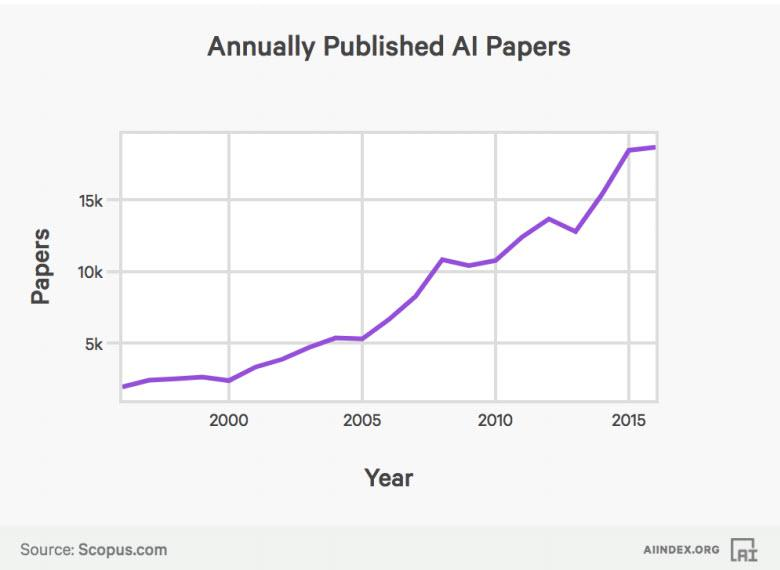
\includegraphics[width=5cm]{figures/annually-published-papers}
\end{subfigure}%
\begin{subfigure}{.5\textwidth}
  \centering
  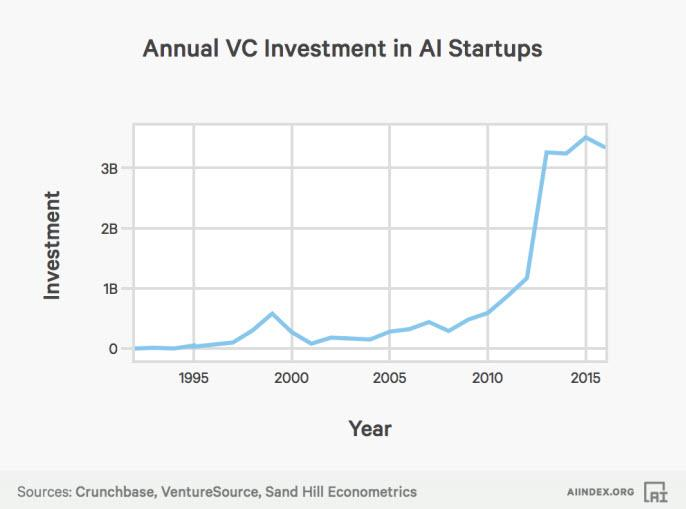
\includegraphics[width=5cm]{figures/annual-VC-investment-in-AI-startups}
\end{subfigure}
\end{figure}
\begin{figure}
\centering
\begin{subfigure}{.5\textwidth}
  \centering
  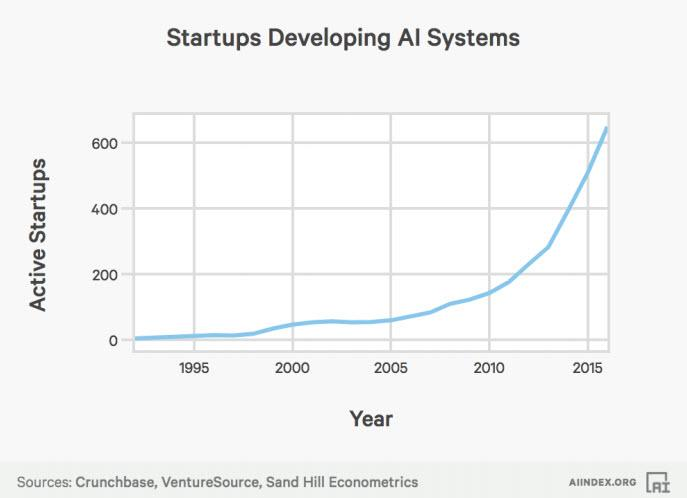
\includegraphics[width=5cm]{figures/startups-developing-ai-systems}
\end{subfigure}%
\begin{subfigure}{.5\textwidth}
  \centering
  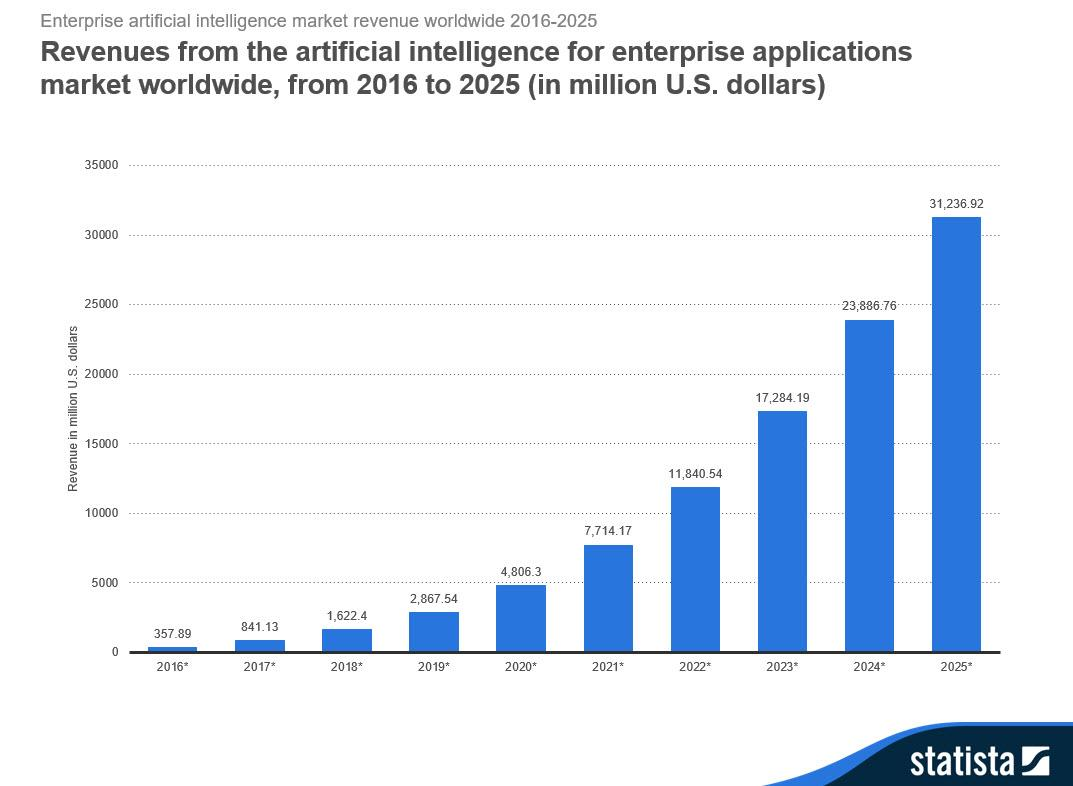
\includegraphics[width=5cm]{figures/AI-for-enterprise-Apps}
\end{subfigure}
\end{figure}
\end{frame}

\begin{frame}{Introduction}
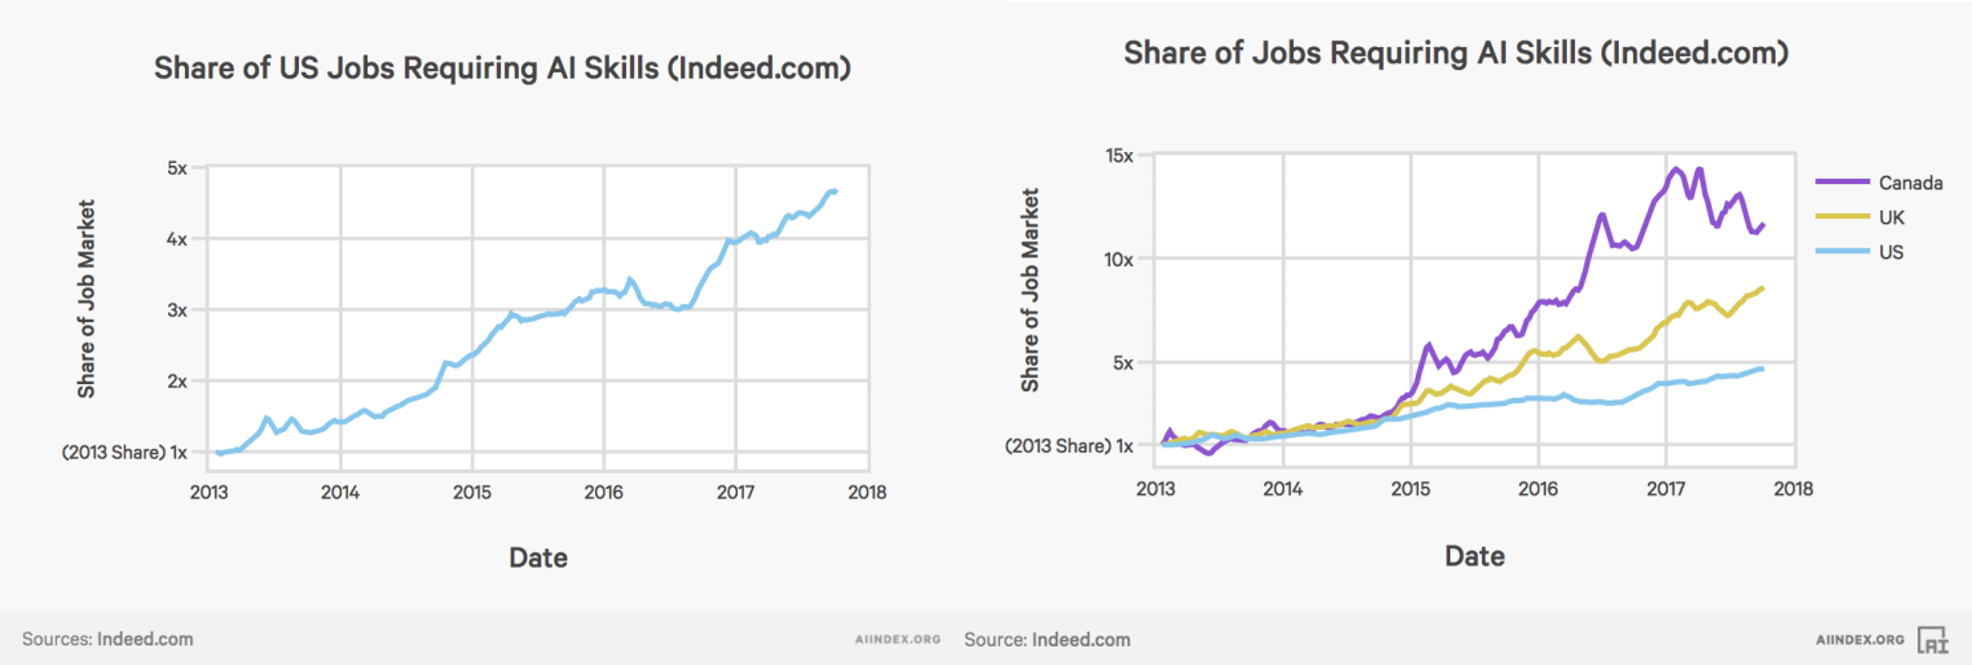
\includegraphics[width=10cm]{figures/AI-Jobs-Composite-Graphic}
\begin{figure}
\centering
\begin{subfigure}{.5\textwidth}
  \centering
  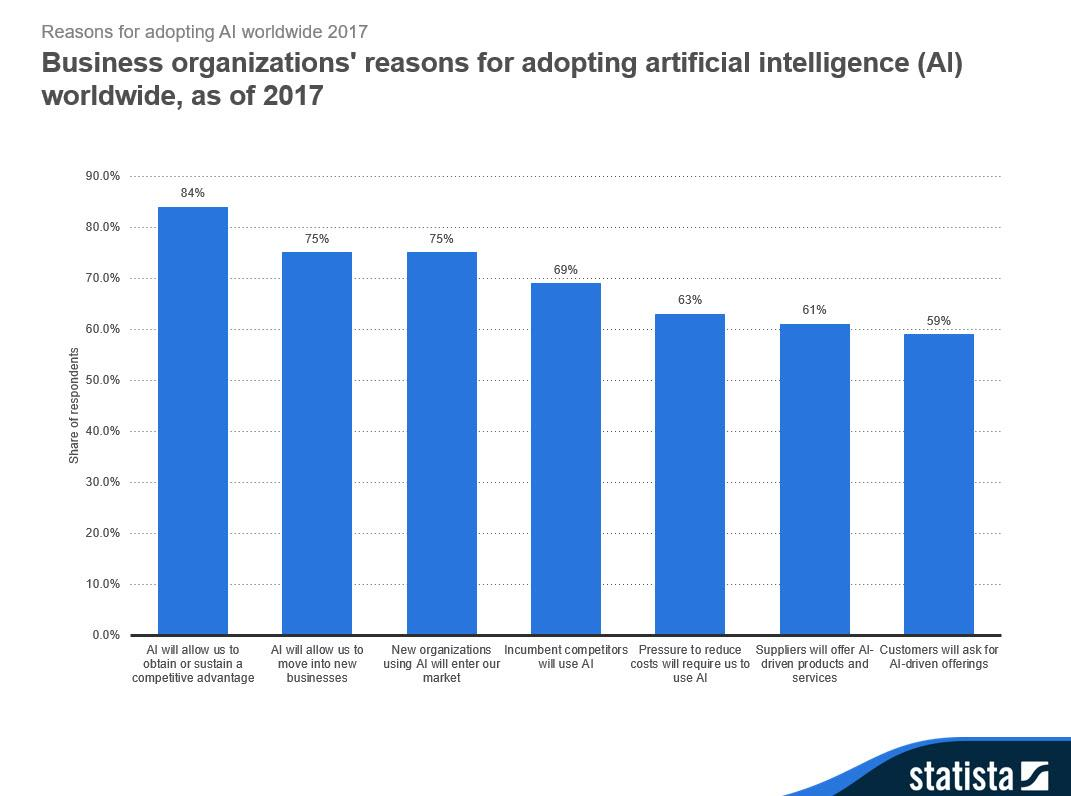
\includegraphics[width=5cm]{figures/Reasons-for-adopting-AI-Worldwide}
\end{subfigure}%
\begin{subfigure}{.5\textwidth}
  \centering
  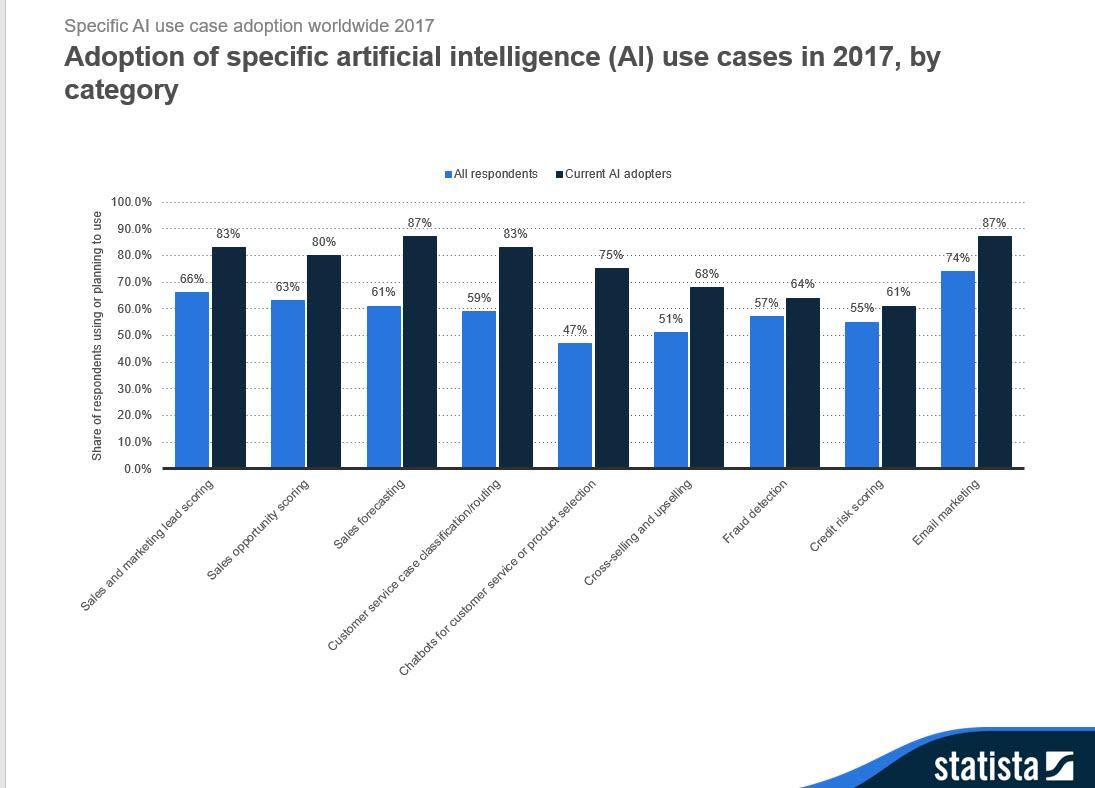
\includegraphics[width=5cm]{figures/Marketing-Centric-Adoption-Use-Cases-of-AI}
\end{subfigure}
\end{figure}
\end{frame}

\begin{frame}{Introduction}
\centering
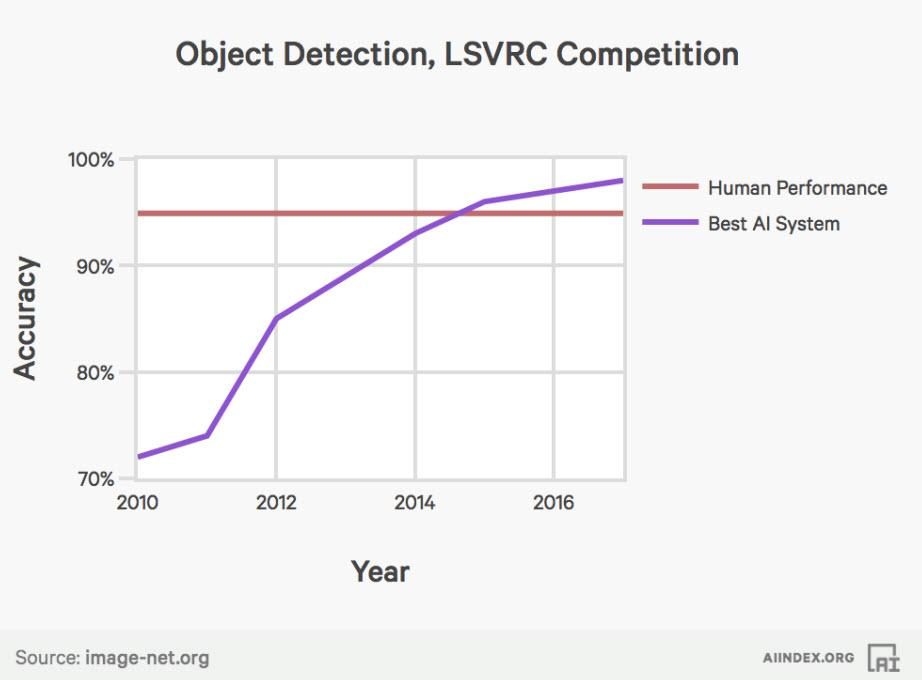
\includegraphics[width=10cm]{figures/Large-Scale-Visual}
\end{frame}

\begin{frame}{AI is almost everywhere today}
\begin{itemize}
\item Cheap and tiny smart devices using AI on the way
\item Google's TensorFlow in use by Airbnb, eBay, Uber, Snapchat, Dropbox, etc.
\item Neural Networks approachable by beginners
\item Slimmed down version can run on phones
\item TensorFlow Lite for embedded devices like printers, fridges, thermostats, speakers, and household gadgets
\item Currently devices are connected and AI tasks are done in the cloud
\item Microsoft and Amazon teamed up to build competitor Gluon
\end{itemize}
\end{frame}

\begin{frame}{Usage areas}
\fontsize{7pt}{5}\selectfont
\begin{figure}
\centering
\begin{subfigure}{.25\textwidth}
  \centering
  Virtual Personal Assistants
  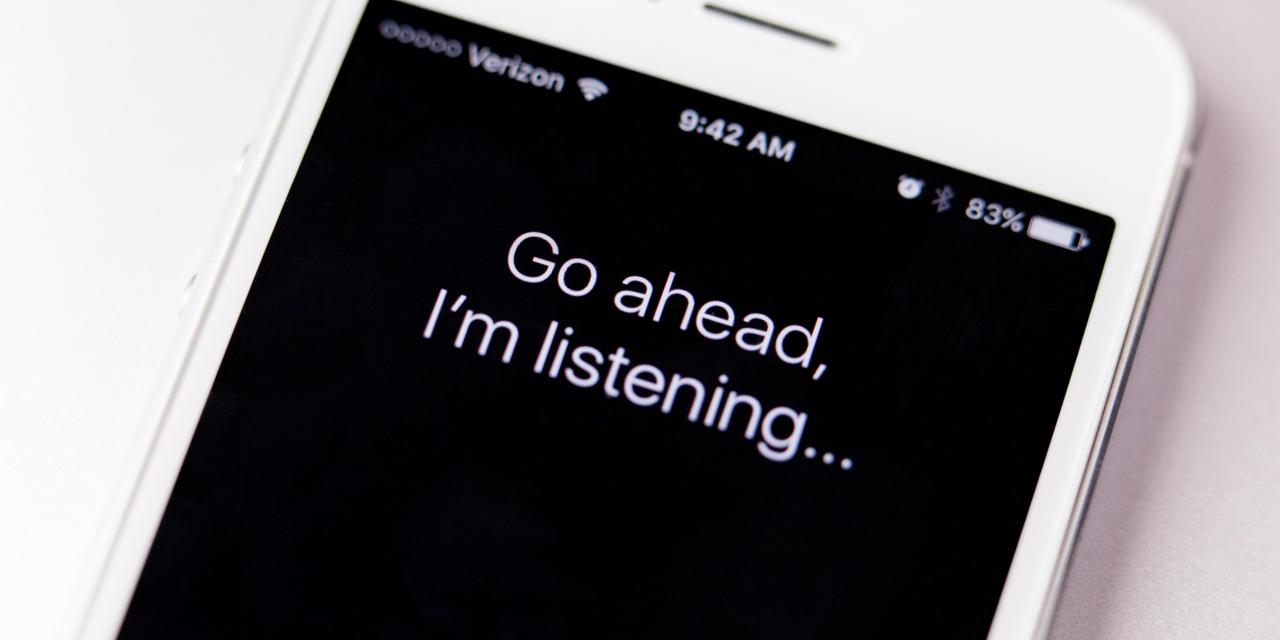
\includegraphics[width=2.5cm]{figures/virtual-personal-assistants}
\end{subfigure}%
\begin{subfigure}{.25\textwidth}
  \centering
  Video Games
  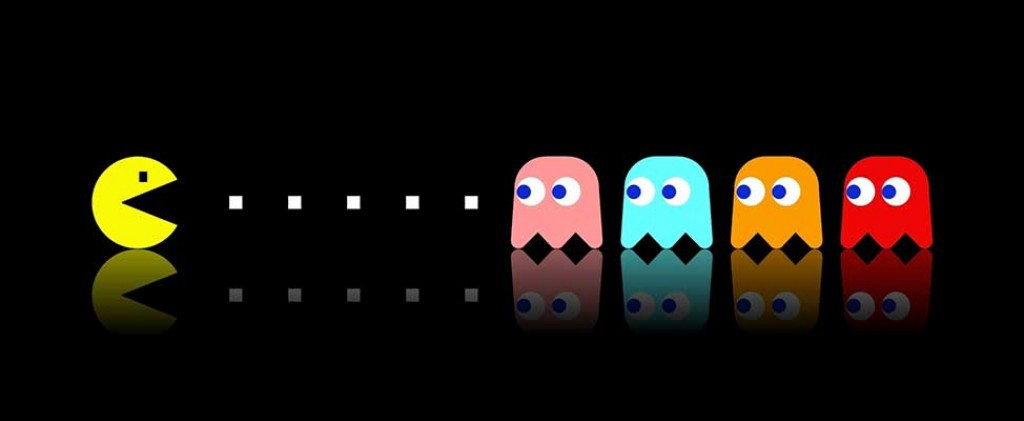
\includegraphics[width=2.5cm]{figures/video-games}
\end{subfigure}
\begin{subfigure}{.25\textwidth}
  \centering
  Smart Cars and Home
  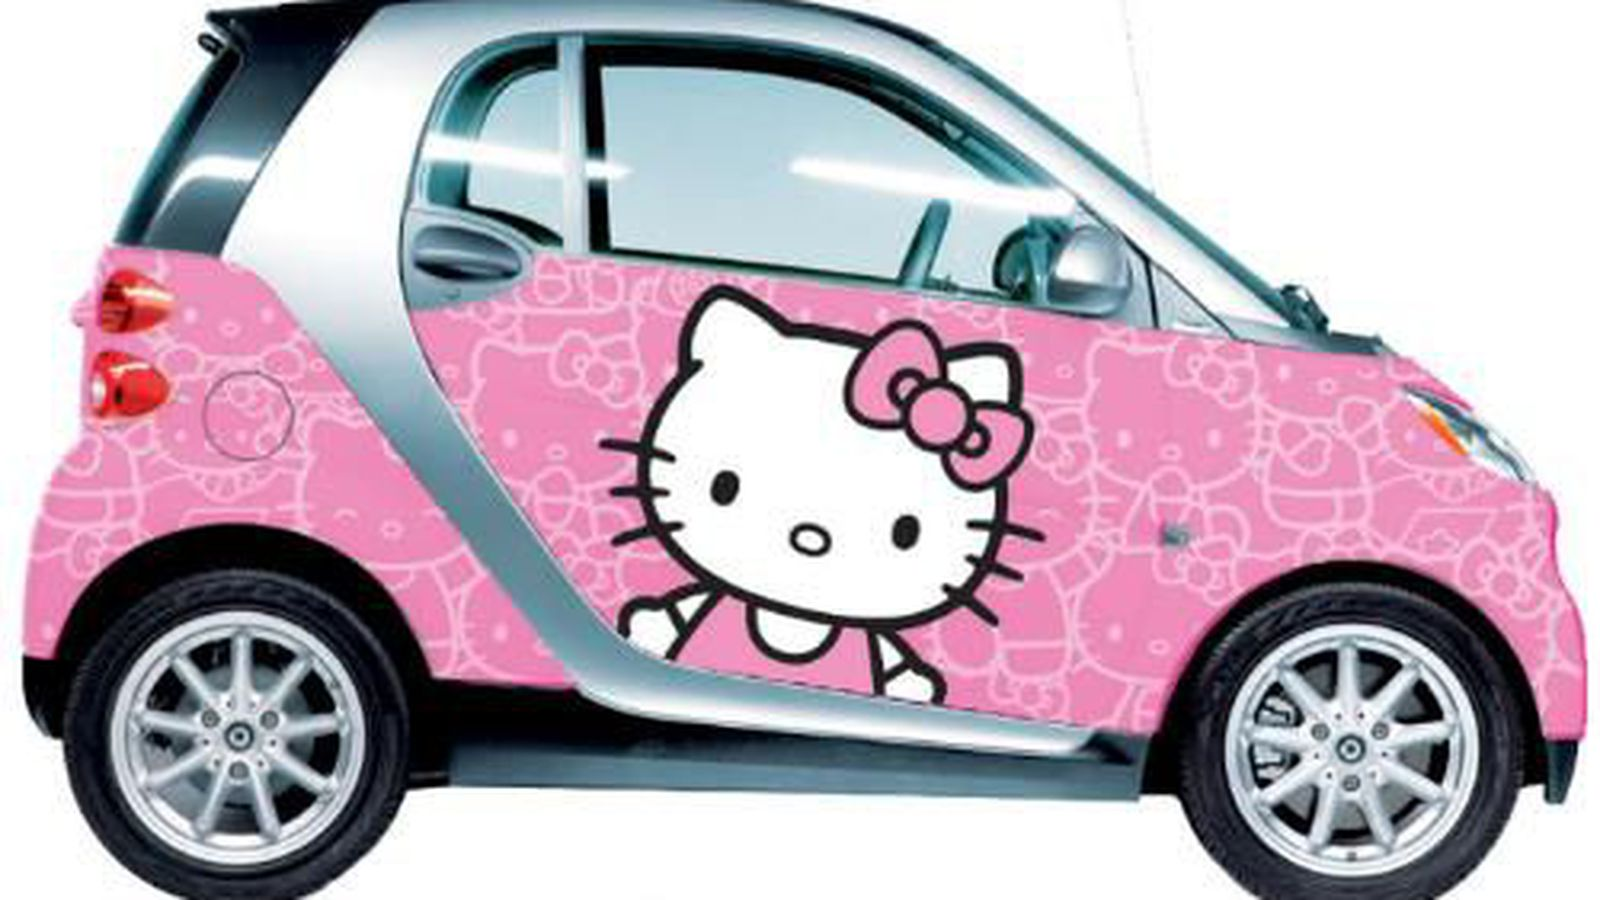
\includegraphics[width=2.5cm]{figures/smart-cars}
\end{subfigure}
\end{figure}
\begin{figure}
\centering
\begin{subfigure}{.25\textwidth}
  \centering
  Purchase Prediction
  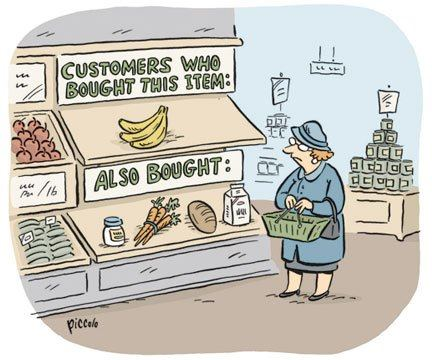
\includegraphics[width=2.5cm]{figures/purchase-prediction}
\end{subfigure}%
\begin{subfigure}{.25\textwidth}
  \centering
  Fraud Detection
  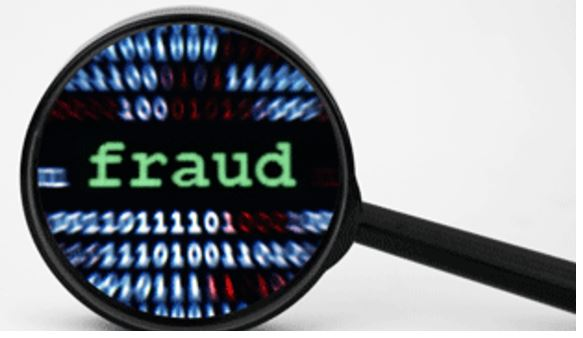
\includegraphics[width=2.5cm]{figures/fraud-detection}
\end{subfigure}
\begin{subfigure}{.25\textwidth}
  \centering
  Online Customer Support
  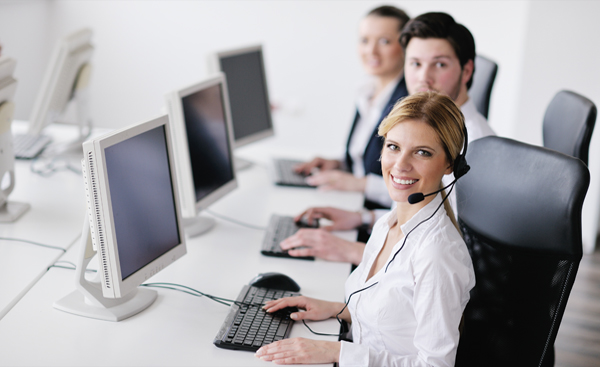
\includegraphics[width=2.5cm]{figures/online-customer-support}
\end{subfigure}
\end{figure}
\begin{figure}
\centering
\begin{subfigure}{.25\textwidth}
  \centering
  News Generation
  
\includegraphics[width=2.5cm]{figures/news-generation}
\end{subfigure}%
\begin{subfigure}{.25\textwidth}
  \centering
  Security Surveillance
  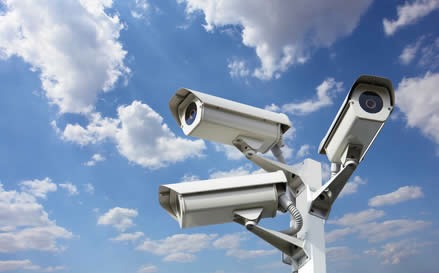
\includegraphics[width=2.5cm]{figures/security-surveillance}
\end{subfigure}
\begin{subfigure}{.25\textwidth}
  \centering
  Media Recommendation
  
\includegraphics[width=2.5cm]{figures/music-and-movie-recommendation}
\end{subfigure}
\end{figure}
\end{frame}

\begin{frame}{Head Spinning Facts and Predictions}
\begin{itemize}
\item 1 billion video cameras connected to AI (NVIDIA Metropolis)
\item 20\% of workforce dedicated to Neural Networks by 2020 (Gartner)
\item 85\% of customer interactions will be managed without humans by 2020 (Gartner)
\item 38\% of jobs in the US could be automated by 2030 (PwC)
\item 60 billion dollars AI market by 2025 (Tractica)
\item 4 billion AI-powered devices in 2017 (IHS Markit)
\item 30,000 lives could be saved each year in the US by AI (Tesla)
\end{itemize}
\end{frame}

\begin{frame}{Global Players}
 \begin{multicols}{2}
 \begin{enumerate}
  \item AIBrain
  \item Amazon
  \item Anki
  \item Apple
  \item Banjo
  \item CloudMinds
  \item Facebook
  \item Google
  \item H2O
  \item IBM
  \item iCarbonX
  \item Intel
  \item Iris AI
  \item Next IT
  \item Salesforce
  \item SoundHound
  \item Twitter
  \item ViSenze
  \item X.ai
  \item Zebra Medical Vision
  \end{enumerate}
  \end{multicols}
\end{frame}

\section{Definition}
\begin{frame}{What are AI and ML?}
\centering
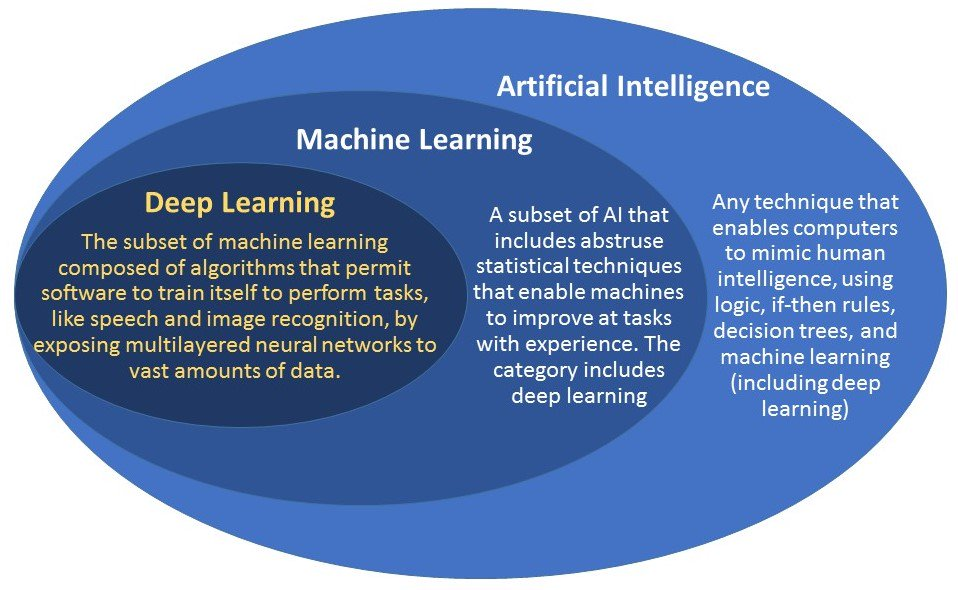
\includegraphics[width=10cm]{figures/ai-ml-dl}
\end{frame}

\begin{frame}{History}
\centering
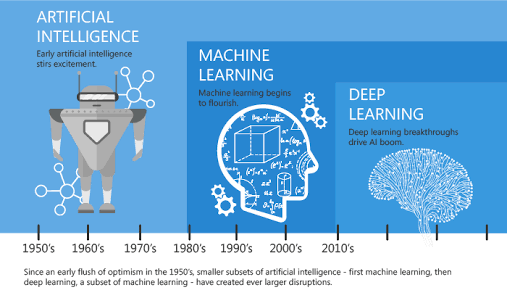
\includegraphics[width=10cm]{figures/history}
\end{frame}

\begin{frame}{Approaches}
\begin{multicols}{2}
\begin{itemize}
\item Supervised Learning
	\begin{itemize}
    \item Classification
    	\begin{itemize}
        \item Identity Fraud Detection
        \item Image Classification
        \item Customer Retention
        \item Diagnostics
        \end{itemize}
    \item Regression
    	\begin{itemize}
        \item Advertising Popularity Prediction
        \item Weather Forecasting
        \item Estimating Life Expectancy
        \item Population Growth Prediction
        \end{itemize}
    \end{itemize}
\item Unsupervised Learning
	\begin{itemize}
    \item Clustering
    	\begin{itemize}
        \item Recommender Systems
        \item Customer Segmentation
        \item Targeted Marketing
        \end{itemize}
    \item Dimensionality Reduction
    	\begin{itemize}
        \item Big Data Visualisation
        \item Meaningful Compression
        \item Structure Discovery
        \item Feature Elicitation
        \end{itemize}
    \end{itemize}
\item Reinforcement Learning
	\begin{itemize}
    \item Game AI
    \item Skill Acquisition
    \item Learning Tasks
    \item Robot Navigation
    \item Real-time Decisions
    \end{itemize}
\end{itemize}
\end{multicols}
\end{frame}

\section{Relation}
\begin{frame}{How AI/ML relate to Big Data and Robotics}
\begin{multicols}{2}
Big Data:
\begin{itemize}
\item Big data analytics in the cloud
\item Hadoop
\item Big data lakes
\item More predictive analytics
\item Better No-SQL
\item Deep Learning
\item In-memory analytics
\end{itemize}
\columnbreak
Robotics:
\begin{itemize}
\item Computer Vision
\item Imitation Learning
\item Self-supervised Learning
\item Assistive and Medical Technologies
\end{itemize}
\end{multicols}
\end{frame}

\section{Sources}
\begin{frame}{Sources of Data}
\begin{itemize}
\item Docs: can exist inside or outside your organization, and like archived data, doesn’t use APIs.
\item Media: exists in-and-out of your organization, may connect with APIs (think an API to collect images from Pinterest and embed them into a product page or email merchandising) and is moderately structured.
\item Business apps: are structured, and using APIs you can pull data from both inside and outside your organization. Internally, think integrating your CRM or Web Content Management with your ecommerce system. Externally, using Weather Co. or Weather Underground data for local personalization is another example.
\item Public web: is external, but some very cool and useful applications can be mashed up with it. For example, is your business affected by the daily fluctuation of currency (or Bitcoin value?), or search term volume that can be pulled from Google Trends?
\end{itemize}
\end{frame}
\section{Sources}
\begin{frame}{Sources of Data}
\begin{itemize}
\item Social media: is high velocity, high volume data that you can use to detect trends, analyze sentiment about your brand, customer service and competitors, or target campaigns to social accounts that match the email addresses in your customer file (to name a few applications).
You’re likely making good use of machine log data through your Web analytics, the next step is using mobile or third party services that help you better identify, target and convert visitors.
\item Sensor data: is high velocity, volume, variety and dare I add…value, when used correctly to understand user context and predict behavior. Sensors for geolocation, temperature, noise, attention, engagement, biometrics, and more can collect reams of data that is useful for better purchase and ownership experiences in a variety of industries.
\item Types: text, voice, images, video - structured or unstructured.
\end{itemize}
\end{frame}

\begin{frame}{GeoDirectory}
Most AI and ML algorithms require location information, which is hence becoming more and more important, therefore GeoDirectory data could be a key variable. \\ \vspace{.5cm}
Examples:
\begin{itemize}
\item Market research, market segmentation 
\item Risk estimation (e.g. mortgages and loans)
\item Spatial patterns of sentiment towards institutions/products 
\item Land use planning 
\item Housing policy and provision
\item Logistics (routing) 
\item Understanding change processes in variety of fields (e.g. health, transport, housing, environment) 
\end{itemize}
\end{frame}

\section{More}
\begin{frame}{How do I find out more?}
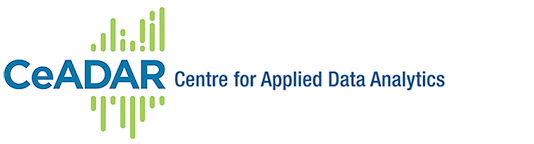
\includegraphics[width=8cm]{figures/ceadar}\\
Website: \url{ceadar.ie} \\

\includegraphics[width=.5cm]{figures/twitter-logo}: \href{https://twitter.com/CeADARIreland}{@CeADARIreland} \\

\includegraphics[width=.5cm]{figures/logo-facebook}: \url{facebook.com/CeADARIreland/} \\

\includegraphics[width=.5cm]{figures/youtube-logo}: \url{youtube.com/user/CeADARIreland/videos} \\

\includegraphics[width=.5cm]{figures/linkedin-logo}: \url{linkedin.com/profile/view?id=231055523} \\ \vspace{.5cm}
CeADAR provides industry prototypes and demonstrators along with state of the art reviews of data analytics technology, tools, best practice methodologies and processes. \\
Main areas: Intelligent Analytic Interfaces, Data Management for Analytics, Advanced Analytics.
\end{frame}

\section{Conclusion}
\begin{frame}{The Future}
\begin{figure}
\centering
\begin{subfigure}{.3\textwidth}
  \centering
  Quantum Computing
  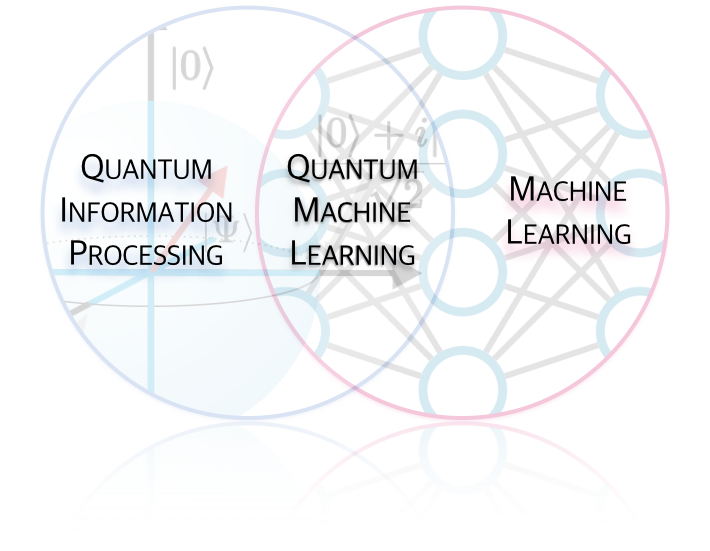
\includegraphics[width=3.5cm]{figures/qml}
\end{subfigure}%
\begin{subfigure}{.3\textwidth}
  \centering
  Better Unsupervised Algorithms
  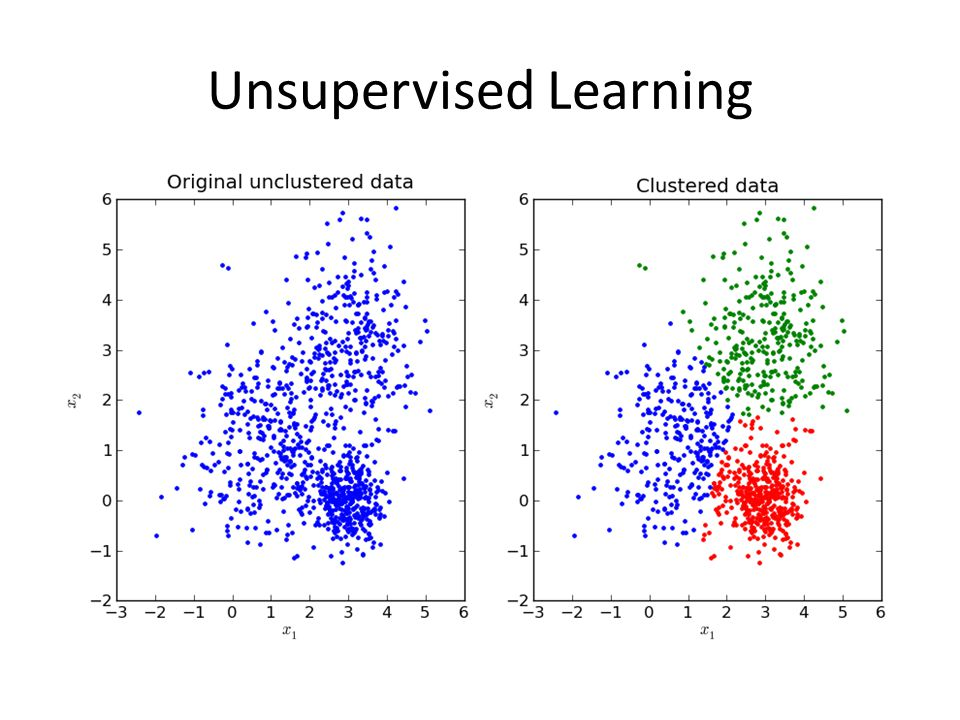
\includegraphics[width=3.5cm]{figures/unsupervised}
\end{subfigure}
\begin{subfigure}{.33\textwidth}
  \centering
	Collaborative Learning
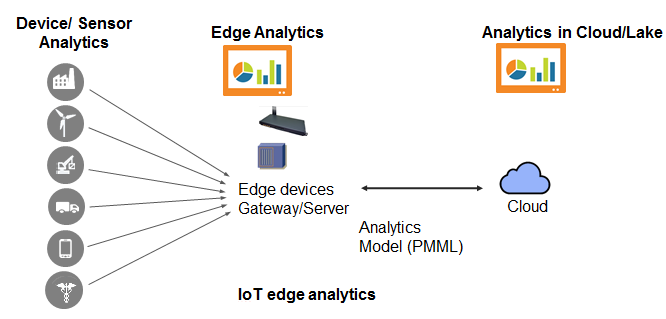
\includegraphics[width=3.5cm]{figures/collaborative}
\end{subfigure}%
\end{figure}
\begin{figure}
\centering
\begin{subfigure}{.4\textwidth}
  \centering
	Deeper Personalisation
	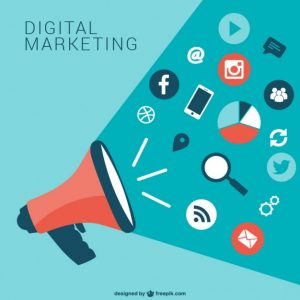
\includegraphics[width=3cm]{figures/personalisation}
\end{subfigure}
\begin{subfigure}{.4\textwidth}
  \centering
  Cognitive Service
  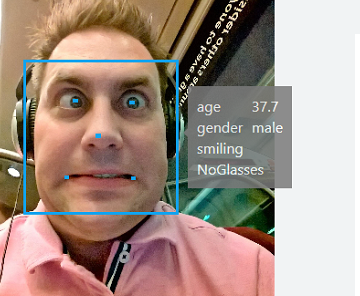
\includegraphics[width=3.5cm]{figures/cognitive}
\end{subfigure}
\end{figure}
\end{frame}

\begin{frame}{Data Flywheels}
\centering
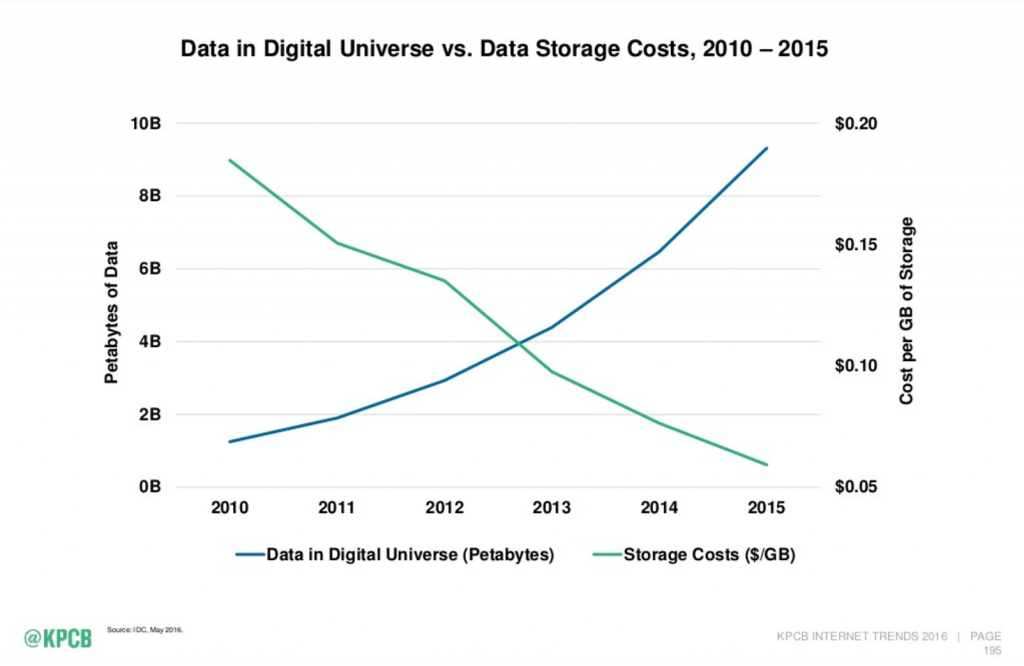
\includegraphics[width=8cm]{data-vs-cost}
\end{frame}

\begin{frame}{The Algorithm Economy}
\centering
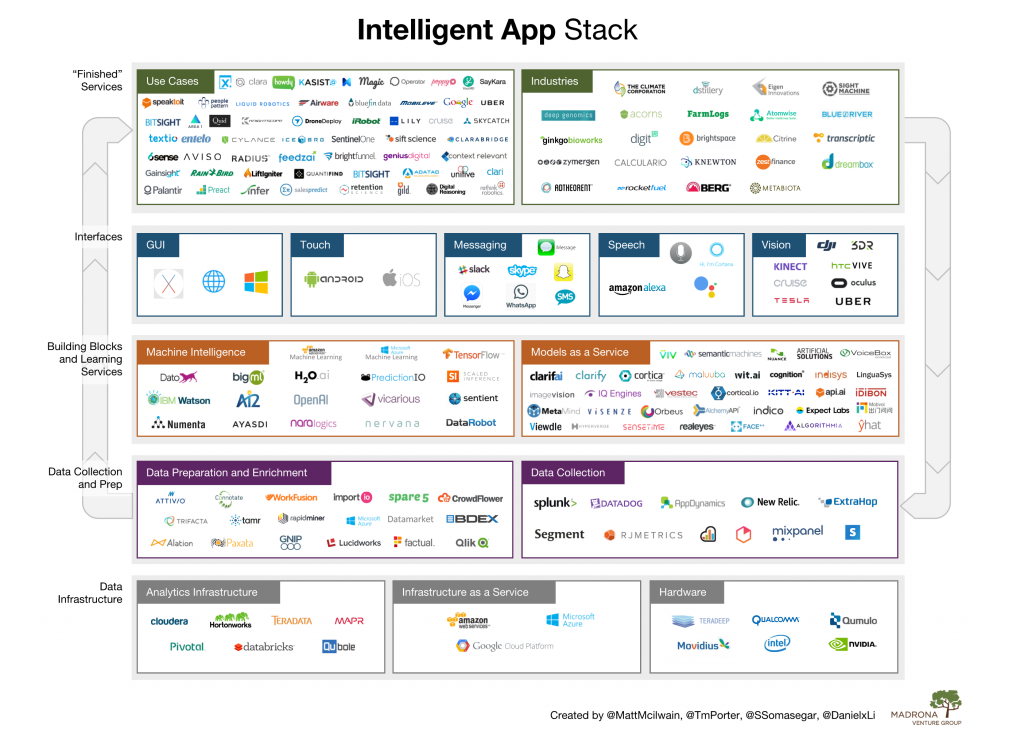
\includegraphics[width=12cm]{figures/intelligent-stack}
\end{frame}

\begin{frame}{Cloud-hosted Intelligence}
\centering
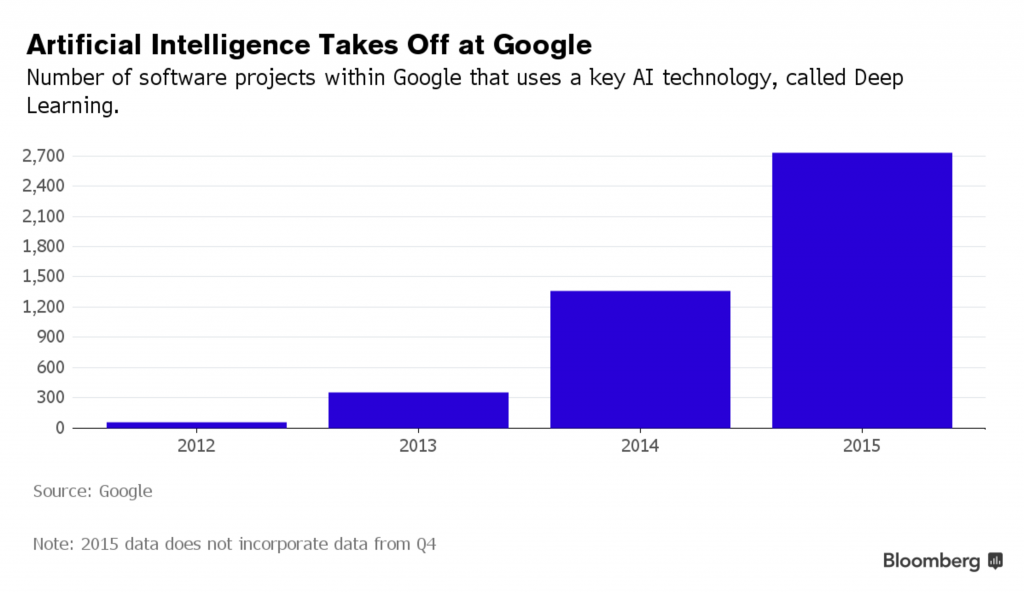
\includegraphics[width=8cm]{figures/cloud-hosted}
\end{frame}

\begin{frame}{Trends}
The confluence of data flywheels, the algorithm economy, and cloud-hosted intelligence means:
\begin{itemize}
\item Every company can now be a data company
\item Every company can now access algorithmic intelligence
\item Every app can now be an intelligent app
\end{itemize}
\end{frame}

\begin{frame}{Who needs ML?}
\textbf{Government agencies} such as public safety and utilities have a particular need for machine learning since they have multiple sources of data that can be mined for insights. Analyzing sensor data, for example, identifies ways to increase efficiency and save money. Machine learning can also help detect fraud and minimize identity theft. \\ \vspace{0.5cm}
\textbf{Geospatial Data Organisations and Businesses:} Imagine being able to train your GIS to perceive and understand the world, and give you insights based on your data. Today, geospatial experts are using machine learning for analyzing big datasets (what do these 2 million points actually mean?) and predictive analytics (e.g. forecasting risk). \\ \vspace{0.5cm}
\textbf{Who else?} Finacial Services, Health Care, Marketing and Sales, Transportation, and many more.
\end{frame}

\begin{frame}{Quotes}
"AI is likely to be either the best or worst thing to happen to humanity."\\ \textbf{Stephen Hawking} \\ \vspace{0.5cm}
"Worth reading Superintelligence by Boston. We need to be super careful with AI. Potentially more dangerous than nukes." \\
\textbf{Elon Musk} \\ \vspace{0.5cm}
"I am in the camp that is concerned about artificial intelligence.  First the machines will do a lot of jobs for us and not be super intelligent.  That should be positive if we manage it well.  A few decades after that though the intelligence is strong enough to be a concern.  I agree with Elon Musk and some others on this and don’t understand why some people are not concerned." \\
\textbf{Bill Gates}

\end{frame}

\begin{frame}{Contact}
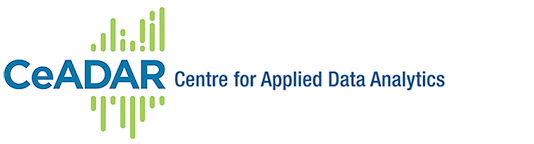
\includegraphics[width=10cm]{figures/ceadar} 
\begin{flushleft}
Bojan Bo\v{z}i\'{c} \\
CeADAR Research Fellow \\
Email: bojan.bozic@dit.ie \\
Twitter: @bojan\_bozic 
\end{flushleft}
\begin{flushleft}
Studies and images from: Gartner, PwC, Tractica, IHS Markit, Tesla, Forbes, MIT Review, quantummachinelearning.org, insidebigdata.com, kdnuggets, martink.me.
\end{flushleft}
\end{frame}

\end{document}